After examining the preference-based consumer theory, we have concluded that if a continuously differentiable demand function $x(\mathbf{p},w)$ is generated by rational preferences, this demand function must have
certain properties (see Thm.\ref{thm:properties_walrasian_demand}) and have a symmetric and negative semidefinite substitution matrix $S(\mathbf{p},w)$. In this section, we would examine the reverse:
if a demand function $x(\mathbf{p},w)$ has these properties, can it be rationalized by some preferences?

\subsection{Recover Preferences from Demand Functions}\label{chp2:sec4:ssec1}
The recovering $\succsim$ from $x(\mathbf{p},w)$ will be done in 2 steps:
\begin{enumerate}
    \item[-] \textbf{Step 1}: recover $e(\mathbf{p},u)$ from $x(\mathbf{p},w)$
    \item[-] \textbf{Step 2}: recover $\succsim$ from $e(\mathbf{p},u)$  
\end{enumerate}
Here, demand is assumed to be single-valued.

\subsubsection*{Recover $e(\mathbf{p},u)$ from $x(\mathbf{p},w)$}
The first step is to recover $e(\mathbf{p},u)$ given a Walrasian demand function $x(\mathbf{p},w)$ that has the assumed properties: satisfies Walras' law, homogeneous of degree 0(see Thm.\ref{thm:properties_walrasian_demand}).
And, demand is assumed to be single-valued.

\subsubsection*{Recover $\succsim$ from $e(\mathbf{p},u)$}
The second step is to recover $\succsim$ given an expenditure function $e(\mathbf{p},u)$ that has the assumed properties: continuous, strictly increasing in $u$, non-decreasing, homogeneous of degree 1, and concave in $\mathbf{p}$ (see Thm.\ref{thm:properties_expenditure_func}).
Since demand is single-valued, $e(\mathbf{p},u)$ is also differentiable.

Here, let $V_u\subset \mathbb{R}^L$  be an at-least-as-good-as set for each utility level $u$ s.t. $e(\mathbf{p},u)$ is the minimal expenditure required for a bundle in $V_u$ at price $\mathbf{p}\gg  0$, i.e. 
$$
e(\mathbf{p},u)=\min_{\mathbf{x}\geq 0}\mathbf{p}\cdot \mathbf{x}\ \text{ s.t. }\mathbf{x}\in V_u
$$

Intuitively, the set $V_u = \left\{ \mathbf{x} \in\mathbb{R}^L_+\mid \mathbf{p}\cdot \mathbf{x}\geq e(\mathbf{p},u),\forall \mathbf{p}\gg 0 \right\}$ satisfies the requirement, that is 
\begin{proposition}{At-least-as-good-as set $V_u$}{atleastasgoodasset_exp}
    For $e(\mathbf{p},u)$ that is strictly increasing in $u$, continuous, non-decreasing, homogeneous of degree 1, concave and differentiable in $\mathbf{p}$, then $\forall u$, $e(\mathbf{p},u)$ is the expenditure function associated with the at-least-as-good-as set
    $$
    V_u = \left\{ \mathbf{x}\in\mathbb{R}^L_+\mid \mathbf{p}\cdot\mathbf{x}\geq e(\mathbf{p},u),\forall \mathbf{p}\gg 0 \right\}
    $$
    i.e. $e(\mathbf{p},u)=\min\left\{ \mathbf{p}\cdot \mathbf{x}\mid \mathbf{x}\in V_u \right\},\forall \mathbf{p}\gg 0$.
\end{proposition}

\textbf{Proof}: Immediately by definitions, $e(\mathbf{p},u)\leq \min\left\{\mathbf{p}\cdot\mathbf{x}\mid \mathbf{x}\in V_n\right\}$. Next, prove $e(\mathbf{p},u)\geq \min\left\{\mathbf{p}\cdot\mathbf{x}\mid \mathbf{x}\in V_n\right\}$: since $e(\mathbf{p},u)$ is concave in $\mathbf{p}$, we have
$$
e(\mathbf{p}',u)\leq e(\mathbf{p},u)+\nabla_{\mathbf{p}}e(\mathbf{p},u)\cdot(\mathbf{p}'-\mathbf{p}),\forall \mathbf{p},\mathbf{p}'
$$
since $e(\mathbf{p},u)$ is homogeneous of degree 1, by Euler's formula, $e(\mathbf{p},u)=\mathbf{p}\cdot\nabla_{\mathbf{p}}e(\mathbf{p},u)$, hence $e(\mathbf{p}',u)\leq \mathbf{p}'\cdot \nabla_{\mathbf{p}}e(\mathbf{p},u),\forall \mathbf{p}'$, plus the fact that $\nabla_{\mathbf{p}(\mathbf{p},u)}\geq 0$, gives that $\nabla_{\mathbf{p}(\mathbf{p},u)}\in V_u$.
By the definition of the at-least-as-good-as set $V_u$, we have $\min\left\{\mathbf{p}\cdot\mathbf{x}\mid \mathbf{x}\in V_u\right\}\leq \mathbf{p}\cdot \nabla_{\mathbf{p}(\mathbf{p},u)}=e(\mathbf{p},u)$. The proof is finished.

With Prop.\ref{prop:atleastasgoodasset_exp}, we can find a set of $V_u$ for each level of $u$, and since $\partial e(\mathbf{p},u)/\partial u>0$, we have $u'>u\Rightarrow V_{u'}\subset V_u$. Each $V_u$ is closed, convex, and bounded below, hence these at-least-as-good-as sets can define a 
preference $\succsim$ (represented by utility levels $u$) that has $e(\mathbf{p},u)$ as its expenditure function (see Fig.\ref{fig:recover_pref_from_exp}).

\begin{figure}[ht]
    \centering
    \caption{Recover $\succsim$ from $e(\mathbf{p},u)$}
    \label{fig:recover_pref_from_exp}
    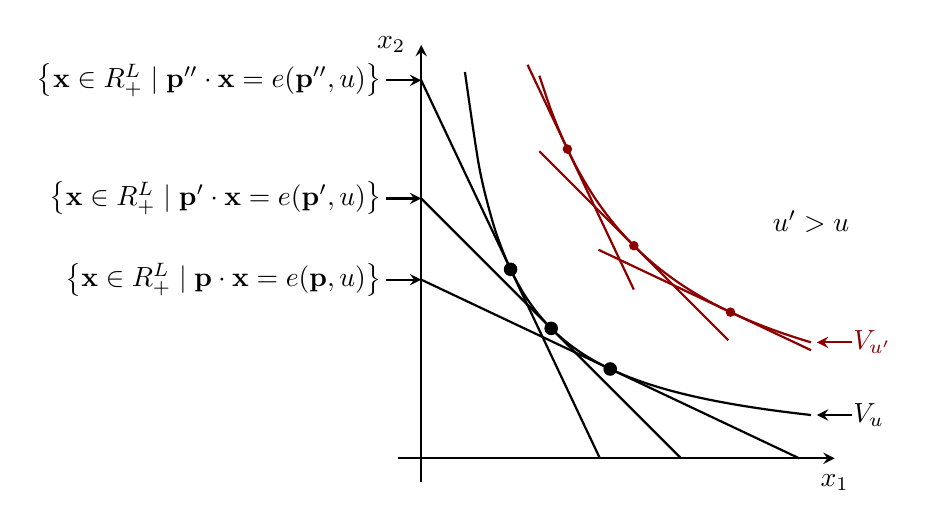
\begin{tikzpicture}[scale=1.5]
        % basics
        \draw [-stealth,color=black,thick] (-0.2,0) -- (3.5,0) node[below=2pt] {$x_1$};
        \draw [-stealth,color=black,thick] (0,-0.2) -- (0,3.5) node[left=2pt] {$x_2$};
        
        % utility and budget lines
        \draw[domain=0.37:3.3, smooth, thick, black, variable=\x] plot ({\x}, {1.1^2/\x}); % utility
        
        \draw[domain=1:3.3, smooth, thick, red!55!black, variable=\x] plot ({\x}, {1.8^2/\x}); % utility'
        
        \draw[domain=0:(4*1.1^2)/3.2, black, thick, variable=\x] plot ({\x}, {3.2-(3.2^2/(4*1.1^2))*\x}); % budget 1
        \draw[domain=0:2.2,black, thick, variable=\x] plot ({\x}, {2.2-\x}); % budget 2
        \draw[domain=0:3.2, black, thick, variable=\x] plot ({\x}, {((4*1.1^2)/3.2)-((4*1.1^2)/3.2^2)*\x}); % budget 3
        
        \draw[domain=0.9:1.8, red!55!black, thick, variable=\x] plot ({\x}, {5.23636-(3.2^2/(4*1.1^2))*\x}); % budget 1'
        \draw[domain=1:2.6,red!55!black, thick, variable=\x] plot ({\x}, {3.6-\x}); % budget 2'
        \draw[domain=1.5:3.3, red!55!black, thick, variable=\x] plot ({\x}, {2.475-((4*1.1^2)/3.2^2)*\x}); % budget 3'
        
        
        
        % bundles
        \filldraw[black] (0.75625,1.1^2/0.75625) circle (1.5pt); % bundle 1
        \filldraw[black] (1.1,1.1) circle (1.5pt); %  bundle 2
        \filldraw[black] (1.1^2/0.75625,0.75625) circle (1.5pt); % bundle 3
         % bundles
        \filldraw[red!55!black] (1.2375,1.8^2/1.2375) circle (1pt); % bundle 1'
        \filldraw[red!55!black] (1.8,1.8) circle (1pt); %  bundle 2'
        \filldraw[red!55!black] (1.8^2/1.2375,1.2375) circle (1pt); % bundle 3'
        
        %% utility
        \draw[stealth-,thick] (3.35,1.1^2/3.3) -- node[right=3pt] {$V_u$} (3.65,1.1^2/3.3);
        \draw[stealth-,thick,red!55!black] (3.35,1.8^2/3.3) -- node[right=3pt] {$V_{u'}$} (3.65,1.8^2/3.3);
        
        % texts and notes
        %% budget change
        \draw[-stealth,thick,black] (-0.3,3.2) -- node[left=4pt] {$\left\{\mathbf{x}\in\mathbb{R}^L_+\mid \mathbf{p}''\cdot\mathbf{x}=e(\mathbf{p}'',u) \right\}$} (0,3.2);
        \draw[-stealth,thick,black] (-0.3,2.2) -- node[left=4pt] {$\left\{\mathbf{x}\in\mathbb{R}^L_+\mid \mathbf{p}'\cdot\mathbf{x}=e(\mathbf{p}',u) \right\}$} (0,2.2);
        \draw[-stealth,thick,black] (-0.3,1.5125) -- node[left=4pt] {$\left\{\mathbf{x}\in\mathbb{R}^L_+\mid \mathbf{p}\cdot\mathbf{x}=e(\mathbf{p},u) \right\}$} (0,1.5125);
        
        \node at (3.3,2) {$u'>u$};
        
    \end{tikzpicture}
\end{figure}

This conclusion can be extended to the case that the underlying preferences of $e(\mathbf{p},u)$ is \textbf{non-convex}. A non-convex $\succsim$ will generate a non-convex 
at-least-as-good-as set, as shown in Fig.\ref{fig:recover_pref_from_exp_nonconvex}.

\begin{figure}[ht]
    \centering
    \caption{Recover non-convex $\succsim$ from $e(\mathbf{p},u)$}
    \label{fig:recover_pref_from_exp_nonconvex}
    \begin{tikzpicture}[scale=1.5]
        % basics
        \draw [-stealth,color=black,thick] (-0.2,0) -- (3.5,0) node[below=2pt] {$x_1$};
        \draw [-stealth,color=black,thick] (0,-0.2) -- (0,3.5) node[left=2pt] {$x_2$};
        
        \draw [thick,red!55!black,tangent=0.9] (0.37,3.3) .. controls (0.5,2.2) and (0.6,1.5) .. (0.8,1.5);
        \draw [black, thick, use tangent] (-1,0) -- (2,0);
        
        \draw [thick,red!55!black,tangent=0.1] (1.5,0.8) .. controls (1.5,0.6) and (2.2,0.5) .. (3.3,0.37);
        \draw [black, thick, use tangent] (-2,0) -- (1,0);
        
        %non-convex part
        \draw [thick,dashed,red!55!black] (0.8,1.5).. controls (1.4,1.4).. (1.5,0.8);
        \draw[domain=0.2:2.05,red!55!black, thick, variable=\x] plot ({\x}, {2.25-\x});
        
        % notes
        %%% actual
        \draw[stealth-,dashed thick,red!55!black] (1.36,1.36) -- node[right=5pt,yshift=10pt,align=left] {Boundary of \textbf{actual} \\ at-least-as-good-as set} (1.7,1.7);
         %%% Slutsky
        \draw[-stealth,thick,black] (1.125-0.4,1.125-0.4) -- node[left=5pt,yshift=-10pt] {Boundary of $V_u$} (1.12,1.12);
        %%% price-utility
        \draw[stealth-,thick,black] (2.05,0.2) -- node[right=5pt] {\scriptsize $\left\{\mathbf{x}\in\mathbb{R}^L_+\mid \mathbf{p}^*\cdot\mathbf{x}=e(\mathbf{p}^*,u^*)\right\}$} (2.4,0.2);
    \end{tikzpicture}
\end{figure}

For this non-convex at-least-as-good-as set, we can always find its convex hull (the solid line) that also generates the
expenditure function $e(\mathbf{p}),u)$. 
Here we have the correspondence between the differentiability of $e(\mathbf{p},u)$ and the , for a specific price-utility pair $(\mathbf{p}^*,u^*)$, there would be more than one expenditure minimizers, and at this price-utility pair $(\mathbf{p}^*,u^*)$,
 the generated $e(\mathbf{p},u)$ would \textbf{NOT} be differentiable. This can be summarized as:
$$
e(\mathbf{p},u) \text{ is differentiable}\Rightarrow \succsim \text{ is convex}
$$

